\chapter{FUNDAMENTAL CONCEPTS}\label{chap:conceitos}

This chapter presents the metrics that will be used for the classifier and provides a brief introduction to the concepts of quantum mechanics required to understand the structure of a quantum computer and how they can be employed in machine-learning tasks.

\section{Evaluation Metrics}

Evaluation metrics play an extremely important role in projects involving machine learning because they allow the progress achieved to be assessed numerically. Machine-learning tasks can be categorized as regression or classification, as can the metrics used for their evaluation. Although several metrics exist for both areas, this section focuses on the most popular evaluation metrics for classification, such as recall, specificity, accuracy, precision, F1-score, and AUC-ROC.

As stated by \citeonline{Métricas}, in the context of binary classification, that is, problems in which each instance belongs to one of two classes, conventionally labelled positive and negative, predictions can be categorized as follows:

\begin{itemize}
\item \textbf{True positive (TP)}: the model predicted that the class was positive, and it was in fact positive;
\item \textbf{True negative (TN)}: the model predicted that the class was negative, and it was in fact negative;
\item \textbf{False positive (FP)}: the model predicted that the class was positive, although it was negative;
\item \textbf{False negative (FN)}: the model predicted that the class was negative, although it was positive;
\end{itemize}

\subsection{Confusion Matrix}

\begin{figure}[H]
\begin{center}
\caption{Confusion matrix.}
\begin{tikzpicture}[
box/.style={draw,rectangle,minimum size=2cm,text width=2cm,align=left}]
\matrix (conmat) [row sep=.1cm,column sep=.1cm] {
\node (tpos) [box,
    label=left:\( \mathbf{p'} \),
    label=above:\( \mathbf{p} \),
    ] {True \\ positive};
&
\node (fneg) [box,
    label=above:\textbf{n},
    label=above right:\textbf{total},
    label=right:\( \mathrm{P}' \)] {False \\ negative};
\\
\node (fpos) [box,
    label=left:\( \mathbf{n'} \),
    label=below left:\textbf{total},
    label=below:P] {False \\ positive};
&
\node (tneg) [box,
    label=right:\( \mathrm{N}' \),
    label=below:N] {True \\ negative};
\\
};
\node [left=.05cm of conmat,text width=1.5cm,align=right] {\textbf{Actual \\ value}};
\node [above=.05cm of conmat] {\textbf{Predicted outcome}};
\end{tikzpicture}
\smallcaption{Source: Author.}
\end{center}
\end{figure}

The confusion matrix summarizes the number of instances in the TP, TN, FP, and FN categories, describing the model's performance. Each row of the matrix represents the instances in an actual class, and each column represents the instances in a predicted class. The confusion matrix is not exactly a metric, but rather a basis on which the results of the metrics are evaluated.

\subsection{Recall}

Recall, or sensitivity, is the fraction of samples from a class that are correctly predicted by the model. It is calculated as the ratio between the true positives and the sum of true positives and false negatives \cite{Métricas}:

\begin{center}
\begin{equation}
\text{Recall} = \dfrac{\text{TP}}{\text{TP} + \text{FN}}
\end{equation}
\end{center}

\subsection{Specificity}

Specificity evaluates the method's ability to identify negative outcomes. It is calculated using the formula \cite{Métricas}:

\begin{center}
\begin{equation}
\text{Specificity} = \dfrac{\text{TN}}{\text{TN} + \text{FP}}
\end{equation}
\end{center}

\subsection{Accuracy}

Accuracy is perhaps the simplest metric to implement and is defined as the number of correct predictions divided by the total number of predictions.

Using the confusion matrix as a basis, the model's accuracy can be obtained with the formula \cite{Métricas}:

\begin{center}
\begin{equation}
\text{Accuracy} = \dfrac{\text{TP} + \text{TN}}{\text{TP} + \text{FP} + \text{FN} + \text{TN}}
\end{equation}
\end{center}

\subsection{Precision}

Precision is the ratio between the true positives and the total predicted positives. It can be obtained using the formula \cite{Métricas}:

\begin{center}
\begin{equation}
\text{Precision} = \dfrac{\text{TP}}{\text{TP} + \text{FP}}
\end{equation}
\end{center}

\subsection{F1-score}

The F1-score combines precision and recall. It is calculated as the harmonic mean of these two metrics. The formula is \cite{Métricas}:

\begin{center}
\begin{equation}
\text{F1-score} = 2 \times \dfrac{\text{Precision} \times \text{Recall}}{\text{Precision} + \text{Recall}}
\end{equation}
\end{center}


\subsection{AUC-ROC}

The ``area under the curve'' (AUC) refers to the area under the ROC curve. This area captures the model's ability to distinguish between positive and negative classes, regardless of the selected cutoff point. A perfect model will have an AUC of 1, whereas a random model (with no discriminatory power) will have an AUC of 0.5.

To calculate the AUC-ROC, the trapezoidal rule is commonly used to approximate the area under the ROC curve. For a binary classification model, the formula for calculating the AUC-ROC is \cite{Métricas}:

\begin{center}
\begin{equation}
\text{AUC ROC} = \int_{0}^{1} \text{Recall}(1-\text{Specificity})\,d(1-\text{Specificity})
\end{equation}
\end{center}

These metrics make it possible to evaluate the performance of a classification model efficiently. Each metric has its own importance and may be more suitable for a particular type of problem or dataset. Therefore, understanding the characteristics and requirements of the problem at hand is essential for selecting the most appropriate metrics to evaluate the model's performance.


\section{Quantum Computing}

%\chapter{CONCEITOS FUNDAMENTAIS}\label{chap:conceitos}

During the first decades of the last century, our understanding of the world changed drastically. The classical deterministic view of mechanics and electrodynamics, which sought to describe all physical phenomena, proved insufficient in light of certain experiments. The quantum hypothesis was first proposed by Max Planck in an attempt to describe the phenomenon of thermal radiation and was subsequently developed by Schrödinger, Dirac \cite{Dirac}, and other physicists.

Quantum mechanics differs from classical theories, and Heisenberg's Uncertainty Principle \cite{Mermin2007QComputerScience} illustrates this difference by stating that measuring the state of a system affects the state of the system itself. In the case of a particle, this means that the position $x$ and the component $p_x=mv_x$ of linear momentum, where $m$ is the mass and $v_x$ is the component of the particle's velocity, cannot be measured simultaneously with arbitrary precision. Instead, the uncertainties $\Delta x$ and $\Delta p$ must satisfy the inequality
\begin{equation} \label{eq:incerteza}
\Delta x \Delta p \geq \frac{\hbar}{2}
\end{equation}
\noindent where $\hbar=h/2\pi$ is Planck's constant divided by $2\pi$.

In quantum mechanics, physical quantities such as $x$ and $p_x$ are represented by linear operators $\hat{x}$ and $\hat{p}_x$, and measurement outcomes correspond to the eigenvalues of these operators \cite{Zubairy2020}. Linear operators can be represented by matrices, and these matrices may not commute, which implies that they do not have common eigenvectors. In this case, measuring one physical quantity affects the measurement of the other. Equation \ref{eq:incerteza} follows from the commutation relation
\begin{equation} \label{eq:heisenberg}
\hat{x}\hat{p}_x - \hat{p}_x \hat{x} = i\hbar
\end{equation}
\noindent between the matrices that represent the physical quantities of position and linear momentum \cite{Zubairy2020}.

In 1981, Richard Feynman and Yuri Manin proposed quantum computers \cite{Wong2022IntroductionClassicalQuantum}, and in 1985, David Deutsch mathematically described the first quantum computer equivalent to a quantum Turing machine \cite{Mermin2007QComputerScience}. Quantum algorithms and computers have since been developed. In short, a quantum computer is a machine whose processing is based on the quantum properties of nature. The following sections address the concepts required to understand how quantum computers operate, as well as quantum machine-learning algorithms.

\subsection{Mathematical Formalism} \label{formalismo}

To understand the concepts underlying quantum computing, we will use the symbolism introduced by Dirac \cite{Dirac}. This notation was created to express states, inner products, and operators in quantum mechanics. The state of a system is described by a vector $\ket{\psi}$, known as a ket and represented by a column matrix, or by a vector $\bra{\psi}$, known as a bra and represented by a row matrix. The inner product between two vectors is a complex number and is denoted by a bra-ket $\braket{\phi | \psi}$. Operators are square matrices constructed from projection operators such as $\ket{\psi}\bra{\phi}$ \cite{Dirac,Mermin2007QComputerScience,Zubairy2020,Wong2022IntroductionClassicalQuantum}.

\subsection{Bits and Qubits} \label{Qubits}

A qubit is the quantum analog of a classical bit. In classical computing, a bit can represent two values, 0 or 1. A qubit, on the other hand, is a quantum system with two basis states represented by the vectors $\ket{0}$ and $\ket{1}$, known as computational-basis states \cite{Nielsen,Mermin2007QComputerScience}.

Unlike classical bits, qubits can be in a state of superposition, which consists of a linear combination of the two computational-basis states:
%
%
\begin{center}
\begin{equation}
\ket{\psi} = \alpha_0\ket{0} + \alpha_1\ket{1} 
\end{equation}
\end{center}
%
%
\noindent where the coefficients $\alpha_0$ and $\alpha_1$ are complex numbers called amplitudes, by analogy with the superposition of waves. Born's rule allows amplitudes to be associated with probabilities \cite{Dirac,Nielsen,Mermin2007QComputerScience,Zubairy2020,Wong2022IntroductionClassicalQuantum}: when a qubit is in the state described by $\ket{\psi}$, the probability that the outcome of a measurement in the computational basis corresponds to the state $\ket{0}$ is $P(0)=|\alpha_0|^2$, whereas the probability that the measurement outcome corresponds to the state $\ket{1}$ is $P(1)=|\alpha_1|^2$. Because the amplitudes $\alpha_0$ and $\alpha_1$ determine probabilities, they must be normalized, that is,
%
%
\begin{center}
\begin{equation}
 |\alpha_0|^2 + |\alpha_1|^2 = 1 
\end{equation}
\end{center}
%
%
\noindent to ensure the proper probabilistic interpretation.

It is important to emphasize that superposition is a unique property of quantum systems and allows a qubit to exist in a state that combines the basis states $\ket{0}$ and $\ket{1}$ \cite{Wong2022IntroductionClassicalQuantum}. This superposition allows quantum computers to process information in parallel, which may give them a potential processing advantage over classical computers.

In a geometric representation, a qubit can be visualized on the Bloch sphere \cite{Wong2022IntroductionClassicalQuantum}, where the pure states $\ket{0}$ and $\ket{1}$ are located at the north and south poles, respectively. Superposition states are represented by points on the surface of the sphere, and the quantum state vector, also known as the Bloch vector, points to the current state of the qubit.

\begin{figure}[H]
\centering
\caption{Bloch sphere.}
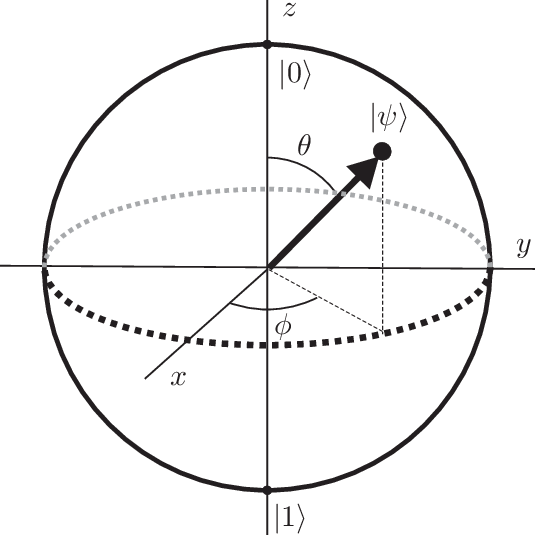
\includegraphics[scale=0.3]{imagens/bloch_sphere.png}
\smallcaption{Source: Wikipedia.}
\label{fig:figura_3}
\end{figure}

The physical representation of a qubit may be the polarization of a photon, the spin state of a particle, two energy levels of an atom or transmon, among other possibilities. Classical computers perform calculations using bit strings, such as 01010. Quantum computers, on the other hand, combine multiple qubits using the tensor product, and therefore the same sequence can be written as:

\begin{center}
\begin{equation}
\ket{\psi} = \ket{0} \otimes \ket{1} \otimes \ket{0} \otimes \ket{1} \otimes \ket{0} = | 01010 \rangle
\end{equation}
\end{center}

It is important to note that a general superposition of five qubits would be:

\begin{center}
\begin{equation}
\ket{\psi} = \alpha_1\ket{00000} + \alpha_2\ket{00001} + \ldots + \alpha_{32}\ket{11111}
\end{equation}
\end{center}

\noindent where $\alpha_i \in \mathbb{C}$ are complex coefficients that satisfy the normalization relation $\sum_{i=1}^{32}|\alpha_i|^2 = 1$ \cite{Wong2022IntroductionClassicalQuantum}.

Entanglement is another unique feature of quantum mechanics that can be used as a resource in quantum computing. To understand entanglement, we must introduce the concept of separable states. For two qubits, a superposition

\begin{center}
\begin{equation}
\ket{\psi} = \alpha_{00}\ket{00} + \alpha_{01}\ket{01} +\alpha_{10}\ket{10} + \alpha_{11}\ket{11}   
\end{equation}
\end{center}

\noindent is separable if it can be written as the tensor product $\ket{\psi_1}\otimes\ket{\psi_2}$ of the states $\ket{\psi_1}$ and $\ket{\psi_2}$, each of which belongs to a vector subspace \cite{Wong2022IntroductionClassicalQuantum}. Thus, the state is separable because it can be written as:

\begin{center}
\begin{equation}
\ket{\psi} = \frac{1}{2}(\ket{00} + \ket{01} - \ket{10} - \ket{11})   
\end{equation}
\end{center}

\begin{center}
\begin{equation}
\ket{\psi} = \left(\frac{1}{\sqrt{2}}(\ket{0} - \ket{1})\right)\otimes\left(\frac{1}{\sqrt{2}}(\ket{0} + \ket{1})\right).
\end{equation}
\end{center}

A characteristic of a separable state such as $\ket{\psi}$ is that knowing the outcome of a measurement performed on one qubit provides no information about the outcome of a measurement performed on the other qubit. In a separable state, the qubits behave as though they were independent of one another.

On the other hand, a Bell state such as

\begin{center}
\begin{equation}\label{eq:Bell}
\ket{\Psi^-} = \frac{1}{\sqrt{2}}(\ket{01} - \ket{10}). 
\end{equation}
\end{center}

is not separable and is called entangled \cite{Wong2022IntroductionClassicalQuantum}. The special characteristic of an entangled state is that the outcomes of measurements performed on one qubit are strongly correlated with the outcomes of measurements performed on the other qubit. For the state $\ket{\Psi^-}$, knowing the outcome of a measurement performed on one qubit makes it possible to predict with absolute certainty the outcome of a measurement performed on the other qubit, even if the two qubits are very far apart when measured. In this case, the qubits are not independent of one another.

\subsection{Quantum Logic Gates} \label{Portas}

Information processing requires the computer to be able to change the state of the qubits that store information. In the circuit model of quantum computing, changes to the state of the qubits are represented by applying a sequence of quantum logic gates to the qubits of the quantum computer \cite{Nielsen}. Quantum gates are linear operators that perform unitary transformations on qubits while preserving the normalization of the states. Because the action of a linear operator $U$ on a superposition is

\begin{center}
\begin{equation}
  U(\alpha_0\ket{0} + \alpha_1\ket{1}) = \alpha_0 U\ket{0} +\alpha_1 U\ket{1},
\end{equation}
\end{center}

\noindent a quantum gate can therefore be characterized by its action on the computational-basis vectors.

The quantum gate $X$, for example, is characterized by:

\begin{center}
\begin{equation}
\begin{aligned}
X\ket{0} &= \ket{1}, \\
X\ket{1} &= \ket{0}.
\end{aligned}
\end{equation}
\end{center}

\noindent corresponding to a quantum generalization of the classical NOT logic gate. In geometric terms, the $X$ gate corresponds to a rotation of $\pi$ of the state vector around the $x$-axis of the Bloch sphere:

\begin{center}
\begin{equation}
X (\alpha_0\ket{0} + \alpha_1\ket{1}) = \alpha_1 \ket{0} + \alpha_0 \ket{1},
\end{equation}
\end{center}

\noindent which corresponds to swapping the amplitudes and, consequently, the probabilities associated with each computational-basis state. Like qubits, quantum gates can be represented in matrix form, as shown for the $X$ gate:

\begin{center}
\begin{equation}
X =
\begin{pmatrix}
0 & 1\\
1 & 0
\end{pmatrix}
\end{equation}
\end{center}

Unlike classical computing, which has only a few one-bit logic gates, quantum computing admits infinitely many single-qubit quantum gates \cite{Nielsen}. Some single-qubit quantum logic gates and their respective matrix and Dirac representations are shown below:

\begin{figure}[H]
    \centering
    \caption{Single-qubit quantum logic gates.}
    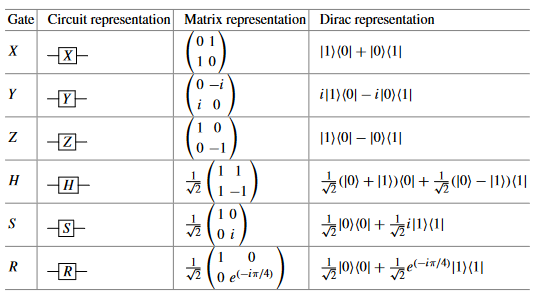
\includegraphics[scale=0.75]{imagens/Tabela_Portas.png}
    \smallcaption{Source: \cite{Schuld2021MLQComputers}.}
    \label{fig:portas_quanticas}
\end{figure}

The $Z$ gate is special because the computational-basis states $\ket{0}$ and $\ket{1}$ are its two eigenstates. The $Z$ gate performs a rotation of $\pi$ around the $z$-axis of the Bloch sphere, reversing the sign of the state $\ket{1}$ \cite{Nielsen}:

\begin{center}
\begin{equation}
Z (\alpha_0\ket{0} + \alpha_1\ket{1}) = \alpha_0 \ket{0} - \alpha_1 \ket{1} = \alpha_0 \ket{0} + e^{i\pi}\alpha_1 \ket{1}.
\end{equation}
\end{center}
\noindent Reversing the sign of the state $\ket{1}$ corresponds to introducing a relative phase of $\pi$ between the two states $\ket{0}$ and $\ket{1}$ in the superposition.

The $Y$ gate, in turn, performs a rotation of $\pi$ around the $y$-axis of the Bloch sphere, changing the state of the qubit as follows \cite{Nielsen}:

\begin{center}
\begin{equation}
Y (\alpha_0\ket{0} + \alpha_1\ket{1}) = -i\alpha_1 \ket{0} + i\alpha_0 \ket{1} = e^{-i\pi/2}(\alpha_1 \ket{0} + e^{i\pi}\alpha_0 \ket{1})
\end{equation}
\end{center}
\noindent which is a combination of the effects of the $X$ and $Z$ gates, swapping the amplitudes and introducing a relative phase between the $\ket{0}$ and $\ket{1}$ components of the superposition.

The $X$, $Y$, and $Z$ gates are called Pauli gates because they are equivalent to the Pauli matrices used to represent spin-$1/2$ particles such as electrons, protons, or neutrons. In addition to the Pauli gates, there are phase gates such as the $S$ and $R$ gates. The $S$ gate introduces a relative phase of $\pi/2$ in the state $\ket{1}$, performing a rotation of $\pi/2$ around the $z$-axis of the Bloch sphere, mapping the state $\ket{0}$ to itself and the state $\ket{1}$ to the state $i\ket{1}$ \cite{Nielsen}.

Finally, the $R$ gate is a general phase gate represented by a diagonal matrix with a parameter $\phi$. It adds a phase $e^{i\phi}$ to the state $\ket{1}$. The $R$ gate also performs a rotation around the $z$-axis of the Bloch sphere, depending on the value of the angle $\phi$ \cite{Nielsen}.

In addition to the Pauli and phase gates, there are rotation gates, which will be important in the development of this work. The $R_x(\theta)$ gate is given in matrix form by

\begin{center}
\begin{equation}
R_x(\theta) =
\begin{pmatrix}
\cos(\theta/2) & -i\sin(\theta/2) \\
-i\sin(\theta/2) & \cos(\theta/2)
\end{pmatrix}
\end{equation}
\end{center}

\noindent and represents a rotation by an angle $\theta$ around the $x$-axis of the Bloch sphere. Similarly, the $R_y(\theta)$ gate, which represents a rotation by an angle $\theta$ around the $y$-axis of the Bloch sphere, is given by

\begin{center}
\begin{equation}
R_y(\theta) =
\begin{pmatrix}
\cos(\theta/2) & -\sin(\theta/2) \\
\sin(\theta/2) & \cos(\theta/2)
\end{pmatrix}
\end{equation}
\end{center}

\noindent and the $R_z(\theta)$ gate is

\begin{center}
\begin{equation}
R_z(\theta) =
\begin{pmatrix}
e^{-i\theta/2} & 0            \\
0              & e^{i\theta/2}
\end{pmatrix}
\end{equation}
\end{center}

\noindent The Pauli gates are special cases of the rotation gates: $X=iR_x(\pi)$, $Y=iR_y(\pi)$, and $Z=iR_z(\pi)$ \cite{Zubairy2020}.

Perhaps the most remarkable single-qubit gate is the $H$ gate, or Hadamard gate. Although the Pauli gates resemble classical logic gates in some respects, the Hadamard gate does not resemble any classical logic gate \cite{Mermin2007QComputerScience}. It can transform a quantum state such as $\ket{0}$ into a uniform superposition, making the probability of measuring 0 equal to the probability of measuring 1. This process can be represented as:

%\begin{equation}
%\begin{centering}
%\begin{quantikz}
%  \lstick{$\ket{1}$} & \gate{H} & \rstick{$\frac{1}{\sqrt{2}}(\ket{0} + \ket{1})$}
%\end{quantikz}
%\end{centering}
%\end{equation}

\begin{equation}
H\ket{0} = \frac{1}{\sqrt{2}}(\ket{0} + \ket{1}).
\end{equation}

\noindent Here, the output of the Hadamard gate is represented by the state $\ket{+} = (\ket{0} + \ket{1})/\sqrt{2}$, which indicates an equally probable superposition of the states $\ket{0}$ and $\ket{1}$. According to Born's rule \cite{Nielsen}, the probabilities of measuring the states $\ket{0}$ and $\ket{1}$ are equal, that is, $P(0) = P(1) = 1/2$. Applying the Hadamard gate to a qubit in the state $\ket{1}$ gives the following transformation:

\begin{equation}
H\ket{1} = \frac{1}{\sqrt{2}}(\ket{0} - \ket{1}),
\end{equation}

\noindent which corresponds to the state $\ket{-} = (\ket{0} - \ket{1})/\sqrt{2}$, another uniform superposition of the states $\ket{0}$ and $\ket{1}$. Because $\braket{-}{+} = 0$, the states $\ket{+}$ and $\ket{-}$ are orthogonal and could be used as an alternative computational basis \cite{Nielsen}.


In addition to single-qubit quantum gates, some quantum gates operate on more than one qubit, such as the $cX$ gate, which is the quantum generalization of the CNOT (controlled-NOT) logic gate, and the Toffoli gate \cite{Nielsen}. The $cX$ gate is a two-qubit gate that acts as a NOT gate on the second qubit if the first qubit is in the state $\ket{1}$. The Toffoli gate, in turn, is a three-qubit gate that acts as a NOT gate on the third qubit if the first two qubits are in the state $\ket{11}$.

These quantum gates play a fundamental role in manipulating and transforming the quantum states of a qubit. They enable complex operations such as superposition, phase inversion, and rotation of quantum states, paving the way for the construction of powerful quantum algorithms and protocols. Understanding quantum gates is fundamental to the development and application of quantum algorithms in machine learning and other areas of quantum computing \cite{Biamonte2017QML, Wong2022IntroductionClassicalQuantum}.

\subsection{Qubit Measurement} \label{Medicao}

Measurement is a fundamental aspect of quantum mechanics and plays a crucial role in quantum computing. According to the postulates of quantum mechanics, measuring an observable $A$, such as position, energy, or linear momentum, will produce one and only one of the eigenvalues of $A$, with the probability determined by the quantum state of the system before the measurement \cite{Nielsen}.

Unlike quantum logic gates, measurement is an irreversible operation that causes the quantum state to collapse. After measurement, the quantum state becomes the eigenvector corresponding to the measured eigenvalue, and all information about the previous superposition and relative phases is lost \cite{Nielsen}.

To illustrate the measurement process, consider the following quantum circuit:

\begin{figure}[H]
\begin{center}
\caption{Example of a quantum circuit.}
\begin{quantikz}
\lstick{$\ket{0}$} & \gate{H} & \ctrl{1} & \meter{} & \rstick{$c_0$} \\
\lstick{$\ket{0}$} & \gate{H} & \targ{}  & \meter{} & \rstick{$c_1$}
\end{quantikz}
\end{center}
\smallcaption{Source: Author.}
\label{fig:circ_quant}
\end{figure}

The circuit above is a simple example that creates an entangled pair of qubits. After creating the entangled pair, the circuit measures the qubits and stores the results in classical bits. The symbol \begin{quantikz}& \meter{} \end{quantikz} indicates a measurement in the circuit.

By executing the circuit several times, it is possible to obtain the probabilities of the states $\ket{0}$ and $\ket{1}$. If the quantum state is an equal superposition of $\ket{0}$ and $\ket{1}$, the probability of measuring each state would be 50\% \cite{Nielsen}. However, because of noise and imperfections in current quantum devices, experimental results may deviate from the ideal theoretical probabilities \cite{Wong2022IntroductionClassicalQuantum}.

Measurement is a fundamental process in quantum computing because it allows useful information to be extracted from quantum states and applied in algorithms and practical applications. However, the irreversible nature of measurement also imposes limitations, such as the destruction of superposition and entanglement. Therefore, developing efficient quantum algorithms and improving quantum devices to reduce the impact of noise are important challenges in quantum-computing research \cite{Schuld2021MLQComputers}.

\section{Input Encoding Method} \label{Encoding}

Encoding classical data in quantum computers is an open problem and depends on the context and the problem under study \cite{Schuld2021MLQComputers}. Several approaches exist for encoding classical information in quantum states, such as basis encoding, amplitude encoding, feature-map encoding, time-evolution encoding, and Hamiltonian encoding. This section addresses only the encoding method used in the development of this project: feature-map encoding.

\subsection{Feature-Map Encoding}

Feature-map encoding is a method for encoding classical data in quantum states that is commonly used in quantum machine learning \cite{Havlicek2019qSupervisedLearning}. In this method, classical data are mapped into a quantum feature space through a nonlinear function. The mapping is designed to preserve and emphasize the properties of the classical data that are relevant to the problem at hand, facilitating the learning process.

One example of a feature map is the transformation of classical data into the rotation angles of quantum rotation gates. Consider a classical data vector $(x_1, x_2)$. To map these data into a quantum feature space, rotation gates are applied to the qubits according to the values $x_1$ and $x_2$. For example, a rotation gate $R_x(\theta_1)$ can be applied to the first qubit using the rotation angle $\theta_1 = \pi x_1$, and a rotation gate $R_y(\theta_2)$ can be applied to the second qubit using the rotation angle $\theta_2 = \pi x_2$. The result is a quantum state that encodes the classical data nonlinearly.

Feature-map encoding is the encoding method used in the development of the classifier in this project. This approach makes it possible to explore quantum properties such as superposition and entanglement and may result in more efficient machine-learning algorithms than classical methods. However, selecting an appropriate feature map is a challenging task and depends on the specific problem under study.

\section{Quantum Machine Learning}

Quantum machine learning is an interdisciplinary field that combines principles and techniques from quantum computing with the field of machine learning. This approach seeks to explore the exponentially greater computational power of quantum systems to improve machine-learning algorithms and models.

In the context of quantum machine learning, traditional concepts are adapted for execution on quantum computers, taking advantage of features such as superposition, entanglement, and quantum interference. These properties allow data to be represented and manipulated in ways that are not possible in classical systems, opening the door to innovative and efficient approaches to solving complex problems.

Several supervised and unsupervised QML algorithms exist, including quantum $k$-means, quantum $k$-median, QPCA, and QSVM. However, this section addresses only QSVM and the variational quantum classifier built on the same encoding, since these are the methods relevant to the classifier developed in this work.

\subsection{Quantum Support Vector Machine (QSVM)} \label{QSVM}

A support vector machine (SVM) is a supervised machine-learning algorithm used for classification and regression. The objective of the algorithm is to find a hyperplane in an $N$-dimensional space (where $N$ is the number of features) that maximizes the separation of points into distinct classes. The hyperplane is defined by the equation:

\begin{equation}
\mathbf{w} \cdot \mathbf{x} + b = 0,
\end{equation}

\noindent where $\mathbf{w}$ is a weight vector, $\mathbf{x}$ is the feature vector, and $b$ is the bias. The classification of a new point is determined by the decision function:

\begin{equation}
f(\mathbf{x}) = \text{sign}(\mathbf{w} \cdot \mathbf{x} + b).
\end{equation}

SVM algorithms use a set of mathematical functions called kernel functions to transform the input data into a higher-dimensional feature space. The kernel function is defined as:

\begin{equation}
K(\mathbf{x}_i, \mathbf{x}_j) = \langle \phi(\mathbf{x}_i), \phi(\mathbf{x}_j) \rangle,
\end{equation}

\noindent where $\phi$ is a mapping function and $\langle \cdot, \cdot \rangle$ denotes the inner product. Several types of kernel functions exist, including linear, nonlinear, polynomial, RBF, and sigmoid functions.

QSVMs were proposed by \citeonline{Rebentrost2014QSVM} and are similar to classical SVMs, but use quantum computing to accelerate the required calculations. This acceleration would depend on the ability of quantum computing to use superposition, which would make it possible to explore the feature space more efficiently. A QSVM is based on calculating the elements of the quantum kernel matrix, defined as:

\begin{equation}
K_{ij} = \langle \psi(\mathbf{x}_i) | \psi(\mathbf{x}_j) \rangle,
\end{equation}

\noindent where $\psi(\mathbf{x})$ is the quantum feature map, that is, the state that encodes the feature vector $\mathbf{x}$.

\subsection{Variational Quantum Classifier (VQC)} \label{VQC}

In the QSVM described above, the quantum computer is used only to estimate the entries of the kernel matrix; the classification itself is carried out by a classical solver. A second approach, introduced by \citeonline{Havlicek2019qSupervisedLearning}, keeps the same quantum feature-space encoding but replaces the kernel matrix with a parameterized quantum circuit, called an \textit{ansatz}, whose gate parameters are learned during training. This model is known as a variational quantum classifier (VQC). Both approaches share the encoding stage and differ in where the learning takes place: in the kernel matrix for the QSVM, and in the circuit parameters for the VQC.

\section{Application in This Project}

In this project, the classification method used is the variational quantum classifier described in Section \ref{VQC}, built on the quantum feature-space encoding presented in Section \ref{QSVM}. This model was chosen because it can be trained directly on current quantum hardware, without the pairwise kernel estimation that the QSVM requires, and because it allows the encoding circuit and the ansatz to be varied independently.